\subsection{Computation of the bimodule vertex}\label{subsec:VecZ2}

\subsection*{Step 1: Compute isomorphism classes of objects and pick a representative.} In general, what we aim for are representations of the annular category of the form
	\begin{figure}[H]
		\centering
		\begin{tikzpicture}[scale=1.2,baseline=(current bounding box.center)]
			\draw (0,0) circle (0.5cm);
			\draw[bwred,line width=0.4mm]
			\foreach \a in {-60, -120} {
				(\a:0.5) -- (\a:1.6)
			};
			\draw ([shift=(-60:1cm)]0,0) arc (-60:90:1cm);
			\draw ([shift=(-120:1.15cm)]0,0) arc (-120:-60:1.15cm);
			\draw ([shift=(240:0.85cm)]0,0) arc (240:90:0.85cm);
			\draw[] (90:0.5) -- (90:1.6);
			\node at (90:.3cm){$a$};\node at (90:1.75cm){$a+x+z$};
			\node at (-1,0.3) {$x$};
			\node at (1.15,0.3) {$z$};
			\node at (0,-1.3) {$y$};
		\end{tikzpicture}.
	\end{figure}
\noindent
According to the figure above, $(*,*,a)\cong(*,*,a+x+z)$ for all possible labels $x,y,z$, so we pick $(*,*,0)$ as a representative.

\subsection*{Step 2: Find primitive idempotents.} To find a representation of the annular category, we need to compute the primitive idempotents, i.e. we need to find morphisms that map $(*,*,0)$ to $(*,*,0)$ which square to themselves and are orthogonal to each other. Additionally, since we want \emph{primitive} idempotents, we need to make sure that they cannot be written as the sum of idempotents.
Candidates for idempotents are the morphism where $x+z=0$:
	\begin{align}
		T_{0,0}:={}&
		\begin{tikzpicture}[scale=1,baseline=(current bounding box.center)]
			\draw (0,0) circle (0.5cm);
			\draw[bwred,line width=0.4mm]
			\foreach \a in {-60, -120} {
				(\a:0.5) -- (\a:1.6)
			};
%			\draw ([shift=(-60:1cm)]0,0) arc (-60:90:1cm);
%			\draw ([shift=(-120:1.15cm)]0,0) arc (-120:-60:1.15cm);
%			\draw ([shift=(240:0.85cm)]0,0) arc (240:90:0.85cm);
			\draw[] (90:0.5) -- (90:1.6);
			\node at (90:.3cm){$0$};\node at (90:1.75cm){$0$};
%			\node at (-1,0.3) {$0$};
%			\node at (1.15,0.3) {$0$};
%			\node at (0,-1.3) {$0$};
		\end{tikzpicture}\\
%		\hspace{5mm}
		T_{0,1}:={}&
		\begin{tikzpicture}[scale=1,baseline=(current bounding box.center)]
		\draw (0,0) circle (0.5cm);
		\draw[bwred,line width=0.4mm]
		\foreach \a in {-60, -120} {
			(\a:0.5) -- (\a:1.6)
		};
%		\draw ([shift=(-60:1cm)]0,0) arc (-60:90:1cm);
		\draw ([shift=(-120:1.15cm)]0,0) arc (-120:-60:1.15cm);
%		\draw ([shift=(240:0.85cm)]0,0) arc (240:90:0.85cm);
		\draw[] (90:0.5) -- (90:1.6);
		\node at (90:.3cm){$0$};\node at (90:1.75cm){$0$};
%		\node at (-1,0.3) {$0$};
%		\node at (1.15,0.3) {$0$};
		\node at (0,-1.3) {$1$};
		\end{tikzpicture}\\
%		\hspace{5mm}
		T_{1,0}:={}&
		\begin{tikzpicture}[scale=1,baseline=(current bounding box.center)]
		\draw (0,0) circle (0.5cm);
		\draw[bwred,line width=0.4mm]
		\foreach \a in {-60, -120} {
			(\a:0.5) -- (\a:1.6)
		};
		\draw ([shift=(-60:1cm)]0,0) arc (-60:90:1cm);
%		\draw ([shift=(-120:1.15cm)]0,0) arc (-120:-60:1.15cm);
		\draw ([shift=(240:0.85cm)]0,0) arc (240:90:0.85cm);
		\draw[] (90:0.5) -- (90:1.6);
		\node at (90:.3cm){$0$};\node at (90:1.75cm){$0$};
		\node at (-1,0.3) {$1$};
		\node at (1.15,0.3) {$1$};
%		\node at (0,-1.3) {$0$};
		\end{tikzpicture}\\
%		\hspace{5mm}
		T_{1,1}:={}&
		\begin{tikzpicture}[scale=1,baseline=(current bounding box.center)]
		\draw (0,0) circle (0.5cm);
		\draw[bwred,line width=0.4mm]
		\foreach \a in {-60, -120} {
			(\a:0.5) -- (\a:1.6)
		};
		\draw ([shift=(-60:1cm)]0,0) arc (-60:90:1cm);
		\draw ([shift=(-120:1.15cm)]0,0) arc (-120:-60:1.15cm);
		\draw ([shift=(240:0.85cm)]0,0) arc (240:90:0.85cm);
		\draw[] (90:0.5) -- (90:1.6);
		\node at (90:.3cm){$0$};\node at (90:1.75cm){$0$};
		\node at (-1,0.3) {$1$};
		\node at (1.15,0.3) {$1$};
		\node at (0,-1.3) {$1$};
		\end{tikzpicture}.
	\end{align}
\noindent
The first morphism can be interpreted as the identity morphism and it obviously squares to itself. It is easy to see that the second and third diagrams square to the first. To square the final morphism, we need to do the following calculation:\vspace{5pt}
	\begin{align*}
		\begin{tikzpicture}[scale=1,baseline=(current bounding box.center)]
			\draw (0,0) circle (0.5cm);
			\draw[bwred,line width=0.4mm]
			\foreach \a in {-60, -120} {
				(\a:0.5) -- (\a:2)
			};
			\draw[] (90:0.5) -- (90:2);
			\draw ([shift=(-60:1cm)]0,0) arc (-60:90:1cm);
			\draw ([shift=(-120:1.15cm)]0,0) arc (-120:-60:1.15cm);
			\draw ([shift=(240:0.85cm)]0,0) arc (240:90:0.85cm);
			\draw ([shift=(240:1.3cm)]0,0) arc (240:90:1.3cm);
			\draw ([shift=(-60:1.45cm)]0,0) arc (-60:90:1.45cm);
			\draw ([shift=(-120:1.6cm)]0,0) arc (-120:-60:1.6cm);
			\node at (90:.3cm){$0$};\node at (90:2.25cm){$0$};
			\node at (-1,0.3) {$1$};
			\node at (1.15,0.3) {$1$};
			\node at (0,-1.35) {$1$};
			\node at (-1.4,0.6) {$1$};
			\node at (1.5,0.6) {$1$};
			\node at (0,-1.8) {$1$};
		\end{tikzpicture}
		&=-\begin{tikzpicture}[scale=1,baseline=(current bounding box.center)]
			\draw (0,0) circle (0.5cm);
			\draw[bwred,line width=0.4mm]
			\foreach \a in {-60, -120} {
				(\a:0.5) -- (\a:2)
			};
			\draw[] (90:0.5) -- (90:2);
			\draw ([shift=(-60:1cm)]0,0) arc (-60:90:1cm);
			\draw ([shift=(-120:1.25cm)]0,0) arc (-120:-60:1.25cm);
			\draw ([shift=(240:0.85cm)]0,0) arc (240:90:0.85cm);
			\draw ([shift=(240:1.15cm)]0,0) arc (240:90:1.15cm);
%			\draw[] ([shift=(240:1.0cm)]0,0) to [bend left=80] ([shift=(90:1.4cm)]0,0);
			\draw ([shift=(-60:1.45cm)]0,0) arc (-60:90:1.45cm);
			\draw ([shift=(-120:1.6cm)]0,0) arc (-120:-60:1.6cm);
			\node at (90:.3cm){$0$};\node at (90:2.25cm){$0$};
			\node at (-1.1,0.8) {$1$};
			\node at (1.15,0.3) {$1$};
			\node at (0,-1.4) {$1$};
			\node at (-0.8,0.6) {$1$};
			\node at (1.5,0.6) {$1$};
			\node at (0,-1.8) {$1$};
		\end{tikzpicture}\\
		&=\begin{tikzpicture}[scale=1,baseline=(current bounding box.center)]
			\draw (0,0) circle (0.5cm);
			\draw[bwred,line width=0.4mm]
			\foreach \a in {-60, -120} {
				(\a:0.5) -- (\a:2)
			};
			\draw[] (90:0.5) -- (90:2);
			\draw ([shift=(240:0.75cm)]0,0) arc (240:90:0.75cm);
			%\draw ([shift=(-60:1.2cm)]0,0) arc (-60:90:1.2cm);
			\draw ([shift=(-60:1cm)]0,0) to [bend right=70] ([shift=(90:1.4cm)]0,0);
			\draw ([shift=(-120:1.5cm)]0,0) arc (-120:-60:1.5cm);
			\draw ([shift=(240:1.1cm)]0,0) arc (240:90:1.1cm);
			%\draw ([shift=(-60:1.6cm)]0,0.2) arc (-60:90:1.6cm);
			\draw ([shift=(-60:1.4cm)]0,0) to [bend right=70] ([shift=(90:1.75cm)]0,0);
			\draw ([shift=(-120:1.8cm)]0,0) arc (-120:-60:1.8cm);
			\node at (90:.3cm){$0$};\node at (90:2.25cm){$0$};
			\node at (0.2,-0.2) {$0$};
			\node at (-0.2,-0.2) {$0$};
			\node at (-1.1,-2) {$0$};
			\node at (1.1,-2) {$0$};
			\node at (-0.9,0.3) {$1$};
			\node at (1.05,0.3) {$1$};
			\node at (0,-1.65) {$1$};
			\node at (-1.2,0.6) {$1$};
			\node at (1.35,0.6) {$1$};
			\node at (0,-2) {$1$};
		\end{tikzpicture}\\
		&=\begin{tikzpicture}[scale=1,baseline=(current bounding box.center)]
			\draw (0,0) circle (0.5cm);
			\draw[bwred,line width=0.4mm]
			\foreach \a in {-60, -120} {
				(\a:0.5) -- (\a:1.6)
			};
			\draw[] (90:0.5) -- (90:1.6);
			\node at (90:.3cm){$0$};\node at (90:1.75cm){$0$};
%			\draw ([shift=(-60:1cm)]0,0) arc (-60:90:1cm);
%			\draw ([shift=(-120:1.15cm)]0,0) arc (-120:-60:1.15cm);
%			\draw ([shift=(240:0.85cm)]0,0) arc (240:90:0.85cm);
%			\node at (0.2,-0.2) {$0$};
%			\node at (-0.2,-0.2) {$0$};
%			\node at (-0.9,-1.6) {$0$};
%			\node at (0.9,-1.6) {$0$};
%			\node at (-1,0.3) {$0$};
%			\node at (1.15,0.3) {$0$};
%			\node at (0,-1.35) {$0$};
		\end{tikzpicture}\vspace{5pt}.
	\end{align*}
Hence, the second candidate does not square to itself but to the first candidate. 
Similar computations show that $T_{a,b}T_{c,d}=T_{a+c,b+d}$. 
However, since the primitive idempotents form an algebra, we can also consider linear combinations of the candidates. Also, because we have four candidates, we know that the algebra is $4$-dimensional. To find out the primitive idempotents from the candidates, it is convenient to find a representation of them in terms of matrices, i.e.\ we need matrices that multiply in the same way as the candidates. As mentioned above, the first candidate is the identity, hence the corresponding matrix is
	\begin{equation}
		M_{0,0}=\begin{pmatrix}
			1 & 0 & 0 & 0\\
			0 & 1 & 0 & 0\\
			0 & 0 & 1 & 0\\
			0 & 0 & 0 & 1\\
		\end{pmatrix}.
	\end{equation}
From this representation it is clear that this candidate is an idempotent, but not a primitive one: $M_{0,0}$ can be written as
	\begin{equation}
	\begin{split}
	\label{eq_M0}
		M_{0,0}={}&
		\begin{pmatrix}
		1 & 0 & 0 & 0\\
		0 & 0 & 0 & 0\\
		0 & 0 & 0 & 0\\
		0 & 0 & 0 & 0\\
		\end{pmatrix}
		+\begin{pmatrix}
		0 & 0 & 0 & 0\\
		0 & 1 & 0 & 0\\
		0 & 0 & 0 & 0\\
		0 & 0 & 0 & 0\\
		\end{pmatrix}\\
		&+
		\begin{pmatrix}
		0 & 0 & 0 & 0\\
		0 & 0 & 0 & 0\\
		0 & 0 & 1 & 0\\
		0 & 0 & 0 & 0\\
		\end{pmatrix}
		+\begin{pmatrix}
		0 & 0 & 0 & 0\\
		0 & 0 & 0 & 0\\
		0 & 0 & 0 & 0\\
		0 & 0 & 0 & 1\\
		\end{pmatrix}
	\end{split}		.
	\end{equation}
The matrix representing the second candidate has to fulfill $M_{0,1}^2=M_{0,0}$, so a possible choice is
	\begin{equation}
		M_{0,1}=\begin{pmatrix}
			1 & 0 & 0 & 0\\
			0 & 1 & 0 & 0\\
			0 & 0 & -1 & 0\\
			0 & 0 & 0 & -1\\
		\end{pmatrix}.
	\end{equation}
	Note that this representation is not unique. Similar matrices can be found for the remaining morphisms.
From \eqref{eq_M0}, we get four candidates for primitive idempotents. They are indeed primitive idempotents in the algebra of $4$-dimensional matrices. To translate them back into annular diagrams, we just need to express them in terms of $M_{a,b}$, which yields
	\begin{align}
	P_{x,y}=\frac{1}{4}\sum_{a,b}(-1)^{ax+by}M_{a,b}
	\end{align}
which is diagrammatically
	\begin{equation}
	\begin{split}
		P_{x,y}=\frac{1}{4}&
		\left(
			\begin{tikzpicture}[scale=1,baseline=(current bounding box.center)]
			\draw (0,0) circle (0.5cm);
			\draw[bwred,line width=0.4mm]
			\foreach \a in {-60, -120} {
				(\a:0.5) -- (\a:1.6)
			};
			%			\draw ([shift=(-60:1cm)]0,0) arc (-60:90:1cm);
			%			\draw ([shift=(-120:1.15cm)]0,0) arc (-120:-60:1.15cm);
			%			\draw ([shift=(240:0.85cm)]0,0) arc (240:90:0.85cm);
			\draw[] (90:0.5) -- (90:1.6);
			\node at (90:.3cm){$0$};\node at (90:1.75cm){$0$};
			%			\node at (-1,0.3) {$0$};
			%			\node at (1.15,0.3) {$0$};
			%			\node at (0,-1.3) {$0$};
			\end{tikzpicture}
			+(-1)^x
			\begin{tikzpicture}[scale=1,baseline=(current bounding box.center)]
			\draw (0,0) circle (0.5cm);
			\draw[bwred,line width=0.4mm]
			\foreach \a in {-60, -120} {
				(\a:0.5) -- (\a:1.6)
			};
%						\draw ([shift=(-60:1cm)]0,0) arc (-60:90:1cm);
			\draw ([shift=(-120:1.15cm)]0,0) arc (-120:-60:1.15cm);
%						\draw ([shift=(240:0.85cm)]0,0) arc (240:90:0.85cm);
			\draw[] (90:0.5) -- (90:1.6);
			\node at (90:.3cm){$0$};\node at (90:1.75cm){$0$};
			%			\node at (-1,0.3) {$0$};
%						\node at (1.15,0.3) {$0$};
						\node at (0,-1.3) {$1$};
			\end{tikzpicture}\right.\\
			&+(-1)^y
			\begin{tikzpicture}[scale=1,baseline=(current bounding box.center)]
			\draw (0,0) circle (0.5cm);
			\draw[bwred,line width=0.4mm]
			\foreach \a in {-60, -120} {
				(\a:0.5) -- (\a:1.6)
			};
									\draw ([shift=(-60:1cm)]0,0) arc (-60:90:1cm);
%			\draw ([shift=(-120:1.15cm)]0,0) arc (-120:-60:1.15cm);
									\draw ([shift=(240:0.85cm)]0,0) arc (240:90:0.85cm);
			\draw[] (90:0.5) -- (90:1.6);
			\node at (90:.3cm){$0$};\node at (90:1.75cm){$0$};
						\node at (-1,0.3) {$1$};
									\node at (1.15,0.3) {$1$};
%			\node at (0,-1.3) {$1$};
			\end{tikzpicture}\\
			&\left.+(-1)^{x+y}
			\begin{tikzpicture}[scale=1,baseline=(current bounding box.center)]
			\draw (0,0) circle (0.5cm);
			\draw[bwred,line width=0.4mm]
			\foreach \a in {-60, -120} {
				(\a:0.5) -- (\a:1.6)
			};
									\draw ([shift=(-60:1cm)]0,0) arc (-60:90:1cm);
			\draw ([shift=(-120:1.15cm)]0,0) arc (-120:-60:1.15cm);
									\draw ([shift=(240:0.85cm)]0,0) arc (240:90:0.85cm);
			\draw[] (90:0.5) -- (90:1.6);
			\node at (90:.3cm){$0$};\node at (90:1.75cm){$0$};
			\node at (-1,0.3) {$1$};
			\node at (1.15,0.3) {$1$};
			\node at (0,-1.3) {$1$};
			\end{tikzpicture}
			\right).
			\end{split}
	\end{equation}
	
\subsection*{Step 3: Check for isomorphism classes of primitive idempotents.} In general, it is possible that the primitive idempotents we just found are isomorphic to each other, which means that there are matrices within the algebra that we can multiply to $P_{0,0}$, for example, and get $P_{1,0}$. The following equation is an example for how this works:
	\begin{equation}
		\begin{pmatrix} 0 & 0 & 0 & 0\\ 1 & 0 & 0 & 0\\ 0 & 0 & 0 & 0\\ 0 & 0 & 0 & 0\\ \end{pmatrix}P_{0,0} \begin{pmatrix} 0 & 1 & 0 & 0\\ 0 & 0 & 0 & 0\\ 0 & 0 & 0 & 0\\ 0 & 0 & 0 & 0\\ \end{pmatrix}=P_{1,0}.\label{eqn:isoids}
	\end{equation}
However, the two matrices we multiply $P_{0,0}$ with are not elements of the matrix algebra (the matrices on the algebra only have entries on the diagonal). If they were elements of the algebra, they would form an isomorphism between $P_{0,0}$ and $P_{1,0}$, so we would pick either $P_{0,0}$ or $P_{1,0}$ as a representative.

This step can be much more complicated for algebras with bigger dimensions. However, there is a nice trick which helps to see how many isomorphism classes there are, which is the Artin-Wedderburn theorem (see, for example, \cite{Beachy1999}). It states that any semi-simple algebra can be decomposed into a direct sum of full matrix algebras, i.e.
	\begin{equation}
		\mathcal{M}\cong\bigoplus\mathcal{M}_d,
	\end{equation}
	where $\dim{\mathcal{M}_d}=d^2$. Within a full matrix algebra we can pick, for example, the primitive idempotent $\mathrm{diag}(1,0,\ldots)$ since the equivalent of the matrices in  \eqref{eqn:isoids} exist. We therefore only get one primitive idempotent for each full matrix algebra. In our case, the algebra is 4 dimensional. The possible decompositions are therefore 
	$\mathcal{M}\cong\mathbb{C}\oplus\mathbb{C}\oplus\mathbb{C}\oplus\mathbb{C}$ and $\mathcal{M}_2$. We found the first decomposition was correct so we get four primitive idempotents (as we showed above). 
	In case of a $5$-dimensional matrix algebra, the possible decompositions are
	\begin{equation}
		\mathcal{M}_{5-\mathrm{dim}}\cong\mathbb{C}\oplus\mathcal{M}_2(\mathbb{C}),
	\end{equation}
	or 
	\begin{equation}
		\mathcal{M}_{5-\mathrm{dim}}\cong5\mathbb{C},
	\end{equation}
so we get two or five primitive idempotents respectively.
	
\subsection*{Step 4: Build the full representation.} After we have found the primitive idempotents of the algebra, we can build the full representation. This is done by putting all possible annuli on the outside of the idempotents, hence finding all the basis vectors for this space, i.e.\ all possible vectors
	\begin{equation}
		\begin{tikzpicture}[scale=1,baseline=(current bounding box.center)]
		\draw (0,0) circle (0.5cm);
		\draw[bwred,line width=0.4mm]
		\foreach \a in {-60, -120} {
			(\a:0.5) -- (\a:1.6)
		};
		\draw ([shift=(-60:1cm)]0,0) arc (-60:90:1cm);
		\draw ([shift=(-120:1.15cm)]0,0) arc (-120:-60:1.15cm);
		\draw ([shift=(240:0.85cm)]0,0) arc (240:90:0.85cm);
		\draw[] (90:0.5) -- (90:1.6);
		\node at (90:.3cm){$0$};\node at (90:1.75cm){$\alpha+\gamma$};
		\node at (-1,0.3) {$\alpha$};
		\node at (1.15,0.3) {$\gamma$};
		\node at (0,-1.4) {$\beta$};
		\end{tikzpicture}.
	\end{equation}
%\noindent
In general, the basis vectors are determined by the choice of $\alpha,\beta$ and $\gamma$, therefore there are up to $2^3=8$ possible basis vectors for each representation. However, it is possible that some of these vectors are linearly dependent, which is the case in our example, as we will see. Putting the general annuli around the primitive idempotents $P_{x,y}$ yields
	\begin{align}
	\begin{split}
	\frac{1}{4}&
	\sum_{a,b}(-1)^{ax+by}
	\begin{tikzpicture}[scale=1,baseline=(current bounding box.center)]
	\draw (0,0) circle (0.5cm);
	\draw[bwred,line width=0.4mm]
	\foreach \a in {-60, -120} {
		(\a:0.5) -- (\a:2)
	};
	\draw[] (90:0.5) -- (90:2);
	\draw ([shift=(-60:1cm)]0,0) arc (-60:90:1cm);
	\draw ([shift=(-120:1.15cm)]0,0) arc (-120:-60:1.15cm);
	\draw ([shift=(240:0.85cm)]0,0) arc (240:90:0.85cm);
	\draw ([shift=(240:1.3cm)]0,0) arc (240:90:1.3cm);
	\draw ([shift=(-60:1.45cm)]0,0) arc (-60:90:1.45cm);
	\draw ([shift=(-120:1.6cm)]0,0) arc (-120:-60:1.6cm);
	\node at (90:.3cm){$0$};\node at (90:2.25cm){$\alpha+\gamma$};
	\node at (-1,0.3) {$b$};
	\node at (1.15,0.3) {$b$};
	\node at (0,-1.35) {$a$};
	\node at (-1.4,0.6) {$\alpha$};
	\node at (1.5,0.6) {$\gamma$};
	\node at (0,-1.8) {$\beta$};
	\end{tikzpicture}\\
	&=
	\frac{1}{4}
	\sum_{a,b}(-1)^{a(x+\alpha+\gamma)+by}
	\begin{tikzpicture}[scale=1,baseline=(current bounding box.center)]
	\draw (0,0) circle (0.5cm);
	\draw[bwred,line width=0.4mm]
	\foreach \a in {-60, -120} {
		(\a:0.5) -- (\a:1.6)
	};
	\draw ([shift=(-60:1cm)]0,0) arc (-60:90:1cm);
	\draw ([shift=(-120:1.15cm)]0,0) arc (-120:-60:1.15cm);
	\draw ([shift=(240:0.85cm)]0,0) arc (240:90:0.85cm);
	\draw[] (90:0.5) -- (90:1.6);
	\node at (90:.3cm){$0$};\node at (90:1.75cm){$\alpha+\gamma$};
	\node[rotate=65] at (-1,0.3) {$\alpha+b$};
	\node[rotate=-65] at (1.15,0.3) {$\gamma+b$};
	\node at (0,-1.3) {$\beta+a$};
	\end{tikzpicture}
	\end{split}\\
	&=
	\frac{(-1)^{(x+\alpha^\prime)\beta+y\gamma}}{4}
	\sum_{a^\prime,b^\prime}(-1)^{a^\prime(x+\alpha^\prime)+b^\prime y}
	\begin{tikzpicture}[scale=1,baseline=(current bounding box.center)]
	\draw (0,0) circle (0.5cm);
	\draw[bwred,line width=0.4mm]
	\foreach \a in {-60, -120} {
		(\a:0.5) -- (\a:1.6)
	};
	\draw ([shift=(-60:1cm)]0,0) arc (-60:90:1cm);
	\draw ([shift=(-120:1.15cm)]0,0) arc (-120:-60:1.15cm);
	\draw ([shift=(240:0.85cm)]0,0) arc (240:90:0.85cm);
	\draw[] (90:0.5) -- (90:1.6);
	\node at (90:.3cm){$0$};\node at (90:1.75cm){$\alpha^\prime$};
	\node[rotate=65] at (-1,0.3) {$\alpha^\prime+b^\prime$};
	\node at (1.15,0.3) {$b^\prime$};
	\node at (0,-1.3) {$a^\prime$};
	\end{tikzpicture}
	\end{align}
which is a vector in the morphism space
	\begin{equation}	
		\begin{tikzpicture}
			\draw[bwred,line width=0.4mm] (0,0) -- (1.5,0);
			\draw (0.75,0) -- (0.75,1) node [pos=1.25]{$\alpha^\prime$};
		\end{tikzpicture}.
	\end{equation}
We now have to find a basis for every one of those morphism spaces, i.e.\ for every choice of $\alpha^\prime$. For fixed representation (fixed, $x,y$), we find a unique vector up to a multiplicative scalar for each $\alpha^\prime$, so each morphism space is one dimensional. We define the basis to be
	\begin{equation}
		\begin{tikzpicture}[scale=1,baseline=(current bounding box.center)]
			\draw[bwred,line width=0.4mm] (0,-.25) -- (.75,0) -- (1.5,-.25);
			\draw (0.75,0) -- (0.75,1) node [pos=1.25] {$\alpha$};
			\node[above,right] at (.75,.15) {$(x,y)$};
		\end{tikzpicture}\equiv
		\frac{1}{4}
		\sum_{a,b}(-1)^{a(x+\alpha)+b y}
		\begin{tikzpicture}[scale=1,baseline=(current bounding box.center)]
		\draw (0,0) circle (0.5cm);
		\draw[bwred,line width=0.4mm]
		\foreach \a in {-60, -120} {
			(\a:0.5) -- (\a:1.6)
		};
		\draw ([shift=(-60:1cm)]0,0) arc (-60:90:1cm);
		\draw ([shift=(-120:1.15cm)]0,0) arc (-120:-60:1.15cm);
		\draw ([shift=(240:0.85cm)]0,0) arc (240:90:0.85cm);
		\draw[] (90:0.5) -- (90:1.6);
		\node at (90:.3cm){$0$};\node at (90:1.75cm){$\alpha$};
		\node[rotate=65] at (-1,0.3) {$\alpha+b$};
		\node at (1.15,0.3) {$b$};
		\node at (0,-1.3) {$a$};
		\end{tikzpicture}.
	\end{equation}
The `inflation trick' developed in \cite{BBJ18,BB19a,BB19b} picks out the representation $P_{0,0}$, and we work with that from here on. This means
	\begin{equation}
	\begin{tikzpicture}[scale=1,baseline=(current bounding box.center)]
	\draw[bwred,line width=0.4mm] (0,-.25) -- (.75,0) -- (1.5,-.25);
	\draw (0.75,0) -- (0.75,1) node [pos=1.25] {$\alpha$};
	\end{tikzpicture}:=
	\frac{1}{4}
	\sum_{a,b}(-1)^{a\alpha}
	\begin{tikzpicture}[scale=1,baseline=(current bounding box.center)]
	\draw (0,0) circle (0.5cm);
	\draw[bwred,line width=0.4mm]
	\foreach \a in {-60, -120} {
		(\a:0.5) -- (\a:1.6)
	};
	\draw ([shift=(-60:1cm)]0,0) arc (-60:90:1cm);
	\draw ([shift=(-120:1.15cm)]0,0) arc (-120:-60:1.15cm);
	\draw ([shift=(240:0.85cm)]0,0) arc (240:90:0.85cm);
	\draw[] (90:0.5) -- (90:1.6);
	\node at (90:.3cm){$0$};\node at (90:1.75cm){$\alpha$};
	\node[rotate=65] at (-1,0.3) {$\alpha+b$};
	\node at (1.15,0.3) {$b$};
	\node at (0,-1.3) {$a$};
	\end{tikzpicture}
	\end{equation}

\subsection*{Step 5: Find associator of the extended category.} After the vertex itself is defined, we want to compute the $F$-symbols related to the new object. 
Our goal is to define a Hamiltonian for the chain which will be of the form
	\begin{equation*}
		\begin{tikzpicture}[scale=1,baseline=(current bounding box.center)]
		\draw (.5,.25)--(.5,.75) node [pos=.5,left]{0};
		\draw [bwred, line width=0.25mm] (0,0) -- (.5,.25) -- (1,0);
		\draw [bwred, line width=0.25mm] (0,1) -- (.5,.75)--(1,1);
		\end{tikzpicture}
		=
		\alpha\ \begin{tikzpicture}[scale=1,baseline=(current bounding box.center)]
			\draw [bwred, line width=0.25mm] (0,0) -- (0,1);
			\draw [bwred, line width=0.25mm] (0.5,0) -- (0.5,1);
		\end{tikzpicture}
		+\beta\ \begin{tikzpicture}[scale=1,baseline=(current bounding box.center)]
			\draw (0,0.5) -- (0.5,0.5);
			\draw [bwred, line width=0.25mm] (0,0) -- (0,1);
			\draw [bwred, line width=0.25mm] (0.5,0) -- (0.5,1);			
		\end{tikzpicture}\ .
	\end{equation*}
To compute $\alpha$ and $\beta$ above, in addition to the action on the spin chain, we will need the full set of $F$-symbols.

From the category $\Vec(\Z/2\Z)$, and the bimodule associators we have
\begin{align}
\left(F_{abc}^{a+b+c}\right)_{a+b,b+c}&=1&&\text{From Example~\ref{example:vecG}:} \\& &&F=+1\nonumber\\
\left(F_{ab*}^*\right)_{a+b,*}&=1&&\text{From \eqref{eqn:L}:} L=+1 \\
\left(F_{a*b}^*\right)_{*,*}&=(-1)^{ab}&&\text{From \eqref{eqn:F1}} \\
\left(F_{*ab}^*\right)_{*,a+b}&=1&&\text{From \eqref{eqn:R}:} R=+1.
\end{align}
\noindent
However, there are still some yet unknown $F$-symbols, namely
\begin{align}
	\left(F_{a**}^{a+b}\right)_{*,b}&=??\\
	\left(F_{*a*}^b\right)_{*,*}&=??\\
	\left(F_{**a}^{a+b}\right)_{b,*}&=??\\
	\left(F_{***}^*\right)_{a,b}&=??.
\end{align}
\noindent	
To compute those, we use the following normalization \cite{Bonderson,BSS08}:
	\begin{equation}
		\begin{tikzpicture}[scale=1.2,baseline=(current bounding box.center)]
			\draw (0,0) to node [left] {$a$} (0,1);
			\draw (0.5,0) to node [right] {$b$} (0.5,1);
		\end{tikzpicture}=\sum_c\ \sqrt{\frac{d_c}{d_a d_b}}\ 
		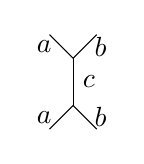
\begin{tikzpicture}[scale=1.2,baseline=(current bounding box.center)]
			\draw (0,0) to node [left] {$a$} (0.25,0.25);
			\draw (0.5,0) to node [right] {$b$} (0.25,0.25);
			\draw (0,1) to node [left] {$a$} (0.25,0.75);
			\draw (0.5,1) to node [right] {$b$} (0.25,0.75);
			\draw (0.25,0.25) to node [right] {$c$} (0.25,0.75);
		\end{tikzpicture}.
	\end{equation}
For the black strings in our diagrams, the sum has only one term and the coefficients are $d_0=1=d_1$, which yields the relation
	\begin{equation}
	\label{eq:completeness}
		\begin{tikzpicture}[scale=1.2,baseline=(current bounding box.center)]
			\draw (0,0) to node [left] {$a$} (0,1);
			\draw (0.5,0) to node [right] {$b$} (0.5,1);
		\end{tikzpicture}=
		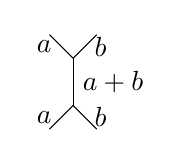
\begin{tikzpicture}[scale=1.2,baseline=(current bounding box.center)]
			\draw (0,0) to node [left] {$a$} (0.25,0.25);
			\draw (0.5,0) to node [right] {$b$} (0.25,0.25);
			\draw (0,1) to node [left] {$a$} (0.25,0.75);
			\draw (0.5,1) to node [right] {$b$} (0.25,0.75);
			\draw (0.25,0.25) to node [right] {$a+b$} (0.25,0.75);
		\end{tikzpicture}.
	\end{equation}
From the fusion rules, $d_*=\sqrt{2}$, so
\begin{equation}
\label{eq:completeness2}
\begin{tikzpicture}[scale=1.2,baseline=(current bounding box.center)]
\draw[bwred,line width=0.4mm] (0,0) to (0,1);
\draw (0.5,0) to node [right] {$a$} (0.5,1);
\end{tikzpicture}=
\begin{tikzpicture}[scale=1.2,baseline=(current bounding box.center)]
\draw[bwred,line width=0.4mm] (0,0) to (0.25,0.25);
\draw (0.5,0) to node [right] {$a$} (0.25,0.25);
\draw[bwred,line width=0.4mm] (0,1) to (0.25,0.75);
\draw (0.5,1) to node [right] {$a$} (0.25,0.75);
\draw[bwred,line width=0.4mm] (0.25,0.25) to (0.25,0.75);
\end{tikzpicture}.
\end{equation}
The computation for $F_{**a}^{a+b}$ is particularly straightforward:
	\begin{align}
		\begin{tikzpicture}[scale=0.7,baseline=(current bounding box.center)]
			\draw[] (0,0) -- (0,1) node[pos=1,above]{$a+b$};
			\draw[] (0,0) -- (-0.707107,-0.707107) node [pos=.5,left] {$b$};
			\draw[bwred,line width=0.4mm] (-0.707107,-0.707107) -- (-1.41421,-1.41421);
			\draw[bwred,line width=0.4mm] (-0.707107,-0.707107) -- (0,-1.41421);
			\draw (0,0) -- (0.707107,-0.707107);
			\draw (0.707107,-0.707107) -- (1.41421,-1.41421);
			\node at (-1.41421,-1.7) {$*$};
			\node at (0,-1.7) {$*$};
			\node at (1.41421,-1.7) {$a$};
		\end{tikzpicture}&=
		\frac{1}{4}\sum_{x,y}(-1)^{bx}
		\begin{tikzpicture}[scale=.75,baseline=(current bounding box.center)]
			\draw (0,0) circle (0.5cm);
			\draw[bwred,line width=0.4mm]
			\foreach \a in {-60, -120} {
				(\a:0.5) -- (\a:1.6)
			};
			\draw[] (90:0.5) -- (90:1.6);
			\draw ([shift=(-60:1cm)]0,0) arc (-60:90:1cm);
			\draw ([shift=(-120:1.15cm)]0,0) arc (-120:-60:1.15cm);
			\draw ([shift=(240:0.85cm)]0,0) arc (240:90:0.85cm);
			\draw[] (0,1.6) -- (0.9,2.1) node[pos=0,left] {$b$};
			\draw[] (0.9,2.1) -- (0.9,2.6);
			\draw (0.9,2.1) -- (2.3,-1.35);
			\node[rotate=60] at (-1,0.3) {$b+y$};
			\node at (1.15,0.3) {$y$};
			\node at (2.3,-1.7) {$a$};
			\node at (0,-1.35) {$x$};
		\end{tikzpicture}
		\\
		=\frac{1}{4}\sum_{x,y}&(-1)^{bx}
		\begin{tikzpicture}[scale=.75,baseline=(current bounding box.center)]
		\draw (0,0) circle (0.5cm);
		\draw[bwred,line width=0.4mm]
		\foreach \a in {-60, -120} {
			(\a:0.5) -- (\a:2.5)
		};
		\draw[] (90:0.5) -- (90:1.6);
		\draw ([shift=(-60:1cm)]0,0) arc (-60:90:1cm);
		\draw ([shift=(-120:1.15cm)]0,0) arc (-120:-60:1.15cm);
		\draw ([shift=(240:0.85cm)]0,0) arc (240:90:0.85cm);
		\draw[] (0,1.6) -- (0.9,2.1) node[pos=0,left] {$b$};
		\draw[] (0.9,2.1) -- (0.9,2.6);
%		\draw (0.9,2.1) -- (2.3,-1.35);
		\draw (-60:1.6) -- (2.3,-2) node[pos=1,below] {$a$};
		\draw (-60:1.4) --(1.5,0) node[right]{$a$} -- (0.9,2.1);
		\node[rotate=60] at (-1,0.3) {$b+y$};
		\node at (1.15,0.3) {$y$};
%		\node at (2.3,-1.7) {$a$};
		\node at (0,-1.35) {$x$};
		%\draw[bwred,line width=0.4mm] (-60:1.6)--(-60:2.5);
		\end{tikzpicture}
		\\
		=\frac{1}{4}\sum_{x,y}&(-1)^{(a+b)x}
		\begin{tikzpicture}[scale=.75,baseline=(current bounding box.center)]
		\draw (0,0) circle (0.5cm);
		\draw[bwred,line width=0.4mm]
		\foreach \a in {-60, -120} {
			(\a:0.5) -- (\a:2.5)
		};
		\draw[] (90:0.5) -- (90:1.6);
		\draw ([shift=(-60:1cm)]0,0) arc (-60:90:1cm);
		\draw ([shift=(-120:1.5cm)]0,0) arc (-120:-60:1.5cm);
		\draw ([shift=(240:0.85cm)]0,0) arc (240:90:0.85cm);
		\draw[] (0,1.6) -- (0.9,2.1) node[pos=0,left] {$b$};
		\draw[] (0.9,2.1) -- (0.9,2.6);
		%		\draw (0.9,2.1) -- (2.3,-1.35);
		\draw (-60:1.6) -- (2.3,-2) node[pos=1,below] {$a$};
		\draw (-60:1.4) --(1.5,0) node[right]{$a$} -- (0.9,2.1);
		\node[rotate=60] at (-1,0.3) {$b+y$};
		\node at (1.15,0.3) {$y$};
		%		\node at (2.3,-1.7) {$a$};
		\node at (0,-1.35) {$x$};
		%\draw[bwred,line width=0.4mm] (-60:1.6)--(-60:2.5);
		\end{tikzpicture}
		\\
		=\frac{1}{4}\sum_{x,y}&(-1)^{(a+b)x}
		\begin{tikzpicture}[scale=.75,baseline=(current bounding box.center)]
		\draw (0,0) circle (0.5cm);
		\draw[bwred,line width=0.4mm]
		\foreach \a in {-60, -120} {
			(\a:0.5) -- (\a:2.5)
		};
		\draw[] (90:0.5) -- (90:1.6) node[pos=1,above]{$a+b$};
		\draw ([shift=(-60:1cm)]0,0) arc (-60:90:1cm);
		\draw ([shift=(-120:1.5cm)]0,0) arc (-120:-60:1.5cm);
		\draw ([shift=(240:0.85cm)]0,0) arc (240:90:0.85cm);
%		\draw[] (0,1.6) -- (0.9,2.1) ;
%		\draw[] (0.9,2.1) -- (0.9,2.6);
		%		\draw (0.9,2.1) -- (2.3,-1.35);
		\draw (-60:1.6) -- (2.3,-2) node[pos=1,below] {$a$};
%		\draw (-60:1.4) --(1.5,0) node[right]{$a$} -- (0.9,2.1);
		\node[rotate=60] at (-1,0.3) {$b+y$};
		\node[rotate=-60] at (1.15,0.3) {$y+a$};
		%		\node at (2.3,-1.7) {$a$};
		\node at (0,-1.35) {$x$};
		%\draw[bwred,line width=0.4mm] (-60:1.6)--(-60:2.5);
		\end{tikzpicture}
		\\
		=\frac{1}{4}\sum_{x,y^\prime}&(-1)^{(a+b)x}
		\begin{tikzpicture}[scale=.75,baseline=(current bounding box.center)]
		\draw (0,0) circle (0.5cm);
		\draw[bwred,line width=0.4mm]
		\foreach \a in {-60, -120} {
			(\a:0.5) -- (\a:2.5)
		};
		\draw[] (90:0.5) -- (90:1.6) node[pos=1,above]{$a+b$};
		\draw ([shift=(-60:1cm)]0,0) arc (-60:90:1cm);
		\draw ([shift=(-120:1.5cm)]0,0) arc (-120:-60:1.5cm);
		\draw ([shift=(240:0.85cm)]0,0) arc (240:90:0.85cm);
		\draw (-60:1.6) -- (2.3,-2) node[pos=1,below] {$a$};
		\node[rotate=60] at (-1,0.3) {$a+b+y^\prime$};
		\node at (1.15,0.3) {$y^\prime$};
		\node at (0,-1.35) {$x$};
		%\draw[bwred,line width=0.4mm] (-60:1.6)--(-60:2.5);
		\end{tikzpicture}
		\\
		&=\begin{tikzpicture}[xscale=-1,scale=0.7,baseline=(current bounding box.center)]
		\draw[] (0,0) -- (0,1) node[pos=1,above]{$a+b$};
		\draw[bwred,line width=0.4mm] (0,0) -- (-0.707107,-0.707107);
		\draw[] (-0.707107,-0.707107) -- (-1.41421,-1.41421);
		\draw[bwred,line width=0.4mm] (-0.707107,-0.707107) -- (0,-1.41421);
		\draw[bwred,line width=0.4mm] (0,0) -- (0.707107,-0.707107);
		\draw[bwred,line width=0.4mm] (0.707107,-0.707107) -- (1.41421,-1.41421);
		\node at (-1.41421,-1.7) {$a$};
		\node at (0,-1.7) {$*$};
		\node at (1.41421,-1.7) {$*$};
		\end{tikzpicture}
	\end{align}
so it follows that 
	\begin{equation}
		\left(F_{**a}^{a+b}\right)_{b,*}=1.
	\end{equation}
The computation of $\left(F_{a**}^{a+b}\right)_{*,b}=1$ is identical. A similar computation yields $\left(F_{*a*}^{b}\right)_{*,*}=(-1)^{ab}$.

Attempting to use \eqref{eq:completeness} to compute $F_{***}^*$ is circular, so we need a different technique. There is an action of a 4-string annular category on the fusion trees on both sides of the equation
\begin{equation}
\begin{split}
\begin{tikzpicture}[scale=0.7,baseline=(current bounding box.center)]
\draw[bwred,line width=0.4mm] (0,0) -- (0,1) node[pos=1,above,text=black]{$*$};
\draw[] (0,0) -- (-0.707107,-0.707107) node [pos=.5,left] {$a$};
\draw[bwred,line width=0.4mm] (-0.707107,-0.707107) -- (-1.41421,-1.41421);
\draw[bwred,line width=0.4mm] (-0.707107,-0.707107) -- (0,-1.41421);
\draw[bwred,line width=0.4mm] (0,0) -- (0.707107,-0.707107);
\draw[bwred,line width=0.4mm] (0.707107,-0.707107) -- (1.41421,-1.41421);
\node at (-1.41421,-1.7) {$*$};
\node at (0,-1.7) {$*$};
\node at (1.41421,-1.7) {$*$};
\end{tikzpicture}
=&
\left(F_{***}^*\right)_{a,0}
\begin{tikzpicture}[xscale=-1,scale=0.7,baseline=(current bounding box.center)]
\draw[bwred,line width=0.4mm] (0,0) -- (0,1) node[pos=1,above,text=black]{$*$};
\draw[] (0,0) -- (-0.707107,-0.707107) node [pos=.5,left] {$0$};
\draw[bwred,line width=0.4mm] (-0.707107,-0.707107) -- (-1.41421,-1.41421);
\draw[bwred,line width=0.4mm] (-0.707107,-0.707107) -- (0,-1.41421);
\draw[bwred,line width=0.4mm] (0,0) -- (0.707107,-0.707107);
\draw[bwred,line width=0.4mm] (0.707107,-0.707107) -- (1.41421,-1.41421);
\node at (-1.41421,-1.7) {$*$};
\node at (0,-1.7) {$*$};
\node at (1.41421,-1.7) {$*$};
\end{tikzpicture}\\
&+
\left(F_{***}^*\right)_{a,1}
\begin{tikzpicture}[xscale=-1,scale=0.7,baseline=(current bounding box.center)]
\draw[bwred] (0,0) -- (0,1) node[pos=1,above,text=black]{$*$};
\draw[] (0,0) -- (-0.707107,-0.707107) node [pos=.5,left] {$1$};
\draw[bwred,line width=0.4mm] (-0.707107,-0.707107) -- (-1.41421,-1.41421);
\draw[bwred,line width=0.4mm] (-0.707107,-0.707107) -- (0,-1.41421);
\draw[bwred,line width=0.4mm] (0,0) -- (0.707107,-0.707107);
\draw[bwred,line width=0.4mm] (0.707107,-0.707107) -- (1.41421,-1.41421);
\node at (-1.41421,-1.7) {$*$};
\node at (0,-1.7) {$*$};
\node at (1.41421,-1.7) {$*$};
\end{tikzpicture}.
\end{split}
\end{equation}
Both sides of the equation transform in the same representation of this 4-string action. We use this to find the $F$-symbols. Consider applying the annulus
\begin{equation}
\begin{tikzpicture}[scale=1,baseline=(current bounding box.center)]
\draw[bwred,line width=0.4mm](-.9,0)--(-.9,-1);
\draw[bwred,line width=0.4mm](0,0)--(0,-1);\draw[bwred,line width=0.4mm](0,.2)--(0,1);
\draw[bwred,line width=0.4mm](.9,0)--(.9,-1);
\draw[rounded corners] (0,.7)--(-1.6,0)--(-.9,-.5)node[pos=.5,left]{$x_0$};
\draw[rounded corners] (0,.9)--(1.6,0)--(.9,-.5)node[pos=.5,right]{$\ x_1$};
\draw[rounded corners] (-.9,-.9)--(0,-.6)node[pos=.5,above]{$x_2$};
\draw[rounded corners] (0,-.9)--(.9,-.6)node[pos=.5,above]{$x_3$};
\draw[rounded corners] (-2,-1) rectangle (2,1);
\filldraw[fill=white,rounded corners] (-1,-.2) rectangle (1,.2);
\end{tikzpicture}\label{eqn:Ftransform}
\end{equation}
to both sides, resolving the vertices where necessary. The equation becomes
\begin{align}
(-&1)^{(a+x_0)(x_1+x_2)}
\begin{tikzpicture}[scale=0.6,baseline=(current bounding box.center)]
\draw[bwred,line width=0.4mm] (0,0) -- (0,1) node[pos=1,above,text=black]{$*$};
\draw[] (0,0) -- (-0.707107,-0.707107) node [pos=.5,left] {$a+x_0+x_3$};
\draw[bwred,line width=0.4mm] (-0.707107,-0.707107) -- (-1.41421,-1.41421);
\draw[bwred,line width=0.4mm] (-0.707107,-0.707107) -- (0,-1.41421);
\draw[bwred,line width=0.4mm] (0,0) -- (0.707107,-0.707107);
\draw[bwred,line width=0.4mm] (0.707107,-0.707107) -- (1.41421,-1.41421);
\node at (-1.41421,-1.7) {$*$};
\node at (0,-1.7) {$*$};
\node at (1.41421,-1.7) {$*$};
\end{tikzpicture}\\[10pt]
%
\begin{split}
=&
\left(F_{***}^*\right)_{a,0}(-1)^{(x_1+x_2)x_3}
\begin{tikzpicture}[xscale=-1,scale=0.6,baseline=(current bounding box.center)]
\draw[bwred,line width=0.4mm] (0,0) -- (0,1) node[pos=1,above,text=black]{$*$};
\draw[] (0,0) -- (-0.707107,-0.707107) node [pos=.5,right] {$x_1+x_2$};
\draw[bwred,line width=0.4mm] (-0.707107,-0.707107) -- (-1.41421,-1.41421);
\draw[bwred,line width=0.4mm] (-0.707107,-0.707107) -- (0,-1.41421);
\draw[bwred,line width=0.4mm] (0,0) -- (0.707107,-0.707107);
\draw[bwred,line width=0.4mm] (0.707107,-0.707107) -- (1.41421,-1.41421);
\node at (-1.41421,-1.7) {$*$};
\node at (0,-1.7) {$*$};
\node at (1.41421,-1.7) {$*$};
\end{tikzpicture}
\\&+
\left(F_{***}^*\right)_{a,1}(-1)^{x_0+(1+x_1+x_2)x_3}
\begin{tikzpicture}[xscale=-1,scale=0.6,baseline=(current bounding box.center)]
\draw[bwred,line width=0.4mm] (0,0) -- (0,1) node[pos=1,above,text=black]{$*$};
\draw[] (0,0) -- (-0.707107,-0.707107) node [pos=.5,right] {$1+x_1+x_2$};
\draw[bwred,line width=0.4mm] (-0.707107,-0.707107) -- (-1.41421,-1.41421);
\draw[bwred,line width=0.4mm] (-0.707107,-0.707107) -- (0,-1.41421);
\draw[bwred,line width=0.4mm] (0,0) -- (0.707107,-0.707107);
\draw[bwred,line width=0.4mm] (0.707107,-0.707107) -- (1.41421,-1.41421);
\node at (-1.41421,-1.7) {$*$};
\node at (0,-1.7) {$*$};
\node at (1.41421,-1.7) {$*$};
\end{tikzpicture}
\end{split}
\\[10pt]
%
\begin{split}
=&(-1)^{(a+x_0)(x_1+x_2)}
	\left(
	\left(F_{***}^*\right)_{a+x_0+x_3,x_1+x_2}
	\begin{tikzpicture}[xscale=-1,scale=0.6,baseline=(current bounding box.center)]
	\draw[bwred,line width=0.4mm] (0,0) -- (0,1) node[pos=1,above,text=black]{$*$};
	\draw[] (0,0) -- (-0.707107,-0.707107) node [pos=.5,right] {$x_1+x_2$};
	\draw[bwred,line width=0.4mm] (-0.707107,-0.707107) -- (-1.41421,-1.41421);
	\draw[bwred,line width=0.4mm] (-0.707107,-0.707107) -- (0,-1.41421);
	\draw[bwred,line width=0.4mm] (0,0) -- (0.707107,-0.707107);
	\draw[bwred,line width=0.4mm] (0.707107,-0.707107) -- (1.41421,-1.41421);
	\node at (-1.41421,-1.7) {$*$};
	\node at (0,-1.7) {$*$};
	\node at (1.41421,-1.7) {$*$};
	\end{tikzpicture}
	\right.
	\\&+
	\left(F_{***}^*\right)_{a+x_0+x_3,1+x_1+x_2}\left.
	\begin{tikzpicture}[xscale=-1,scale=0.6,baseline=(current bounding box.center)]
	\draw[bwred,line width=0.4mm] (0,0) -- (0,1) node[pos=1,above,text=black]{$*$};
	\draw[] (0,0) -- (-0.707107,-0.707107) node [pos=.5,right] {$1+x_1+x_2$};
	\draw[bwred,line width=0.4mm] (-0.707107,-0.707107) -- (-1.41421,-1.41421);
	\draw[bwred,line width=0.4mm] (-0.707107,-0.707107) -- (0,-1.41421);
	\draw[bwred,line width=0.4mm] (0,0) -- (0.707107,-0.707107);
	\draw[bwred,line width=0.4mm] (0.707107,-0.707107) -- (1.41421,-1.41421);
	\node at (-1.41421,-1.7) {$*$};
	\node at (0,-1.7) {$*$};
	\node at (1.41421,-1.7) {$*$};
	\end{tikzpicture}\right)
\end{split}
\end{align}
where in the second step, \eqref{eqn:Ftransform} has been applied to the left-hand side. This equation reduces to
\begin{align}
\left(F_{***}^*\right)_{a,b}&=(-1)^{ab}\left(F_{***}^*\right)_{0,0}.
\end{align}
We cannot fix $\left(F_{***}^*\right)_{0,0}$ by simply asking which representation the vectors transform under, since there is a global rescaling freedom. Our normalization \eqref{eq:completeness} fixes 
\begin{align}
\left(F_{***}^*\right)_{a,b}&=(-1)^{ab}\frac{\varkappa_*}{\sqrt{2}},
\end{align}
where $\varkappa_*=\pm1$ is the \emph{Frobenius-Schur} indicator of $*$.



\subsection*{Step 6: Check if $F$-symbols obey the pentagon equation.} 
%To check whether the maps that we have just defined obey the pentagon equation, we need the full set of $F$-symbols. This means that, in addition to the vertex we have just computed, we also need to compute the vertex
%	\begin{figure}[H]
%		\begin{tikzpicture}
%			\draw[red,line width=0.4mm] (0,0) -- (1.5,0);
%			\draw (0.75,0) -- (0.75,1);
%		\end{tikzpicture}
%	\end{figure}
%\noindent
%Doing the same steps as above yields
%	\begin{equation*}
%		\begin{tikzpicture}[scale=1,baseline=(current bounding box.center)]
%			\draw[red,line width=0.4mm] (0,0) -- (1.5,0);
%			\draw (0.75,0) to node[near end, right] {$\mu$} (0.75,1);
%		\end{tikzpicture}=\frac{1}{4}\sum_{x,y}(-1)^{\mu y}
%		\begin{tikzpicture}[scale=1,baseline=(current bounding box.center)]
%			\draw (0,0) circle (0.5cm);
%			\draw[red,line width=0.4mm]
%			\foreach \a in {-60, -120} {
%				(\a:0.5) -- (\a:1.6)
%			};
%			\draw (90:0.5) to node[near end, right] {$\mu$} (90:1.6);
%			\draw ([shift=(-60:1cm)]0,0) arc (-60:90:1cm);
%			\draw ([shift=(-120:1.15cm)]0,0) arc (-120:-60:1.15cm);
%			\draw ([shift=(240:0.85cm)]0,0) arc (240:90:0.85cm);
%			\node at (0.2,-0.2) {$0$};
%			\node at (-0.2,-0.2) {$0$};
%			\node at (-1,0.3) {$x$};
%			\node at (1.15,0.3) {$x$};
%			\node at (0,-1.35) {$y$};
%		\end{tikzpicture}.
%	\end{equation*}
We now have the full set of $F$-symbols
	\begin{align*}
		\left(F_{abc}^{a+b+c}\right)_{a+b,b+c}&=1\\
		\left(F_{ab*}^*\right)_{a+b,*}&=1\\
		\left(F_{a*b}^*\right)_{*,*}&=(-1)^{ab}\\
		\left(F_{*ab}^*\right)_{*,a+b}&=1\\
		\left(F_{a**}^{a+b}\right)_{*,b}&=1\\
		\left(F_{*a*}^b\right)_{*,*}&=(-1)^{ab}\\
		\left(F_{**a}^{a+b}\right)_{b,*}&=1\\
		\left(F_{***}^*\right)_{a,b}&=\frac{(-1)^{ab}\varkappa_*}{\sqrt{2}},
	\end{align*}
which happen to be the $F$-symbols for the Ising category. 